\subsection{Questions}
Our research embraces 2 research questions:  main research question (RQ1), and 1 additional research question (\textbf{RQ2}). The second question will be explored on the condition that there is enough time.

\textbf{RQ1} - How does energy efficiency differ between native mobile applications and their mobile web counterparts?

To answer to this question, we will have to run the same scenarios on pairs consisting of a native mobile application and its mobile web counterpart. Statistical analysis will be performed to determine whether there is any statistically significant difference.



\textbf{RQ2} - How does the device type affect the difference in energy consumption between native mobile applications and their mobile web counterparts?

To answer this question, we will perform 2 sets of experiments described in \textbf{RQ2}, but one of them has to be on a low-end device, and the other one on a high-end device. Statistical analysis will be performed to determine whether there is any statistically significant difference.


\subsection{Metrics}
We will use the  \textbf{energy \textcolor{blue}{consumption}} to directly answer our research questions. The remaining 3 metrics will supplement our answers with further insight. 
\begin{itemize}
    \item \textbf{Power consumption (W)} - Power consumption of native and web applications while executing the scenario. 	       %measured using Trepn Power Profiler \cite{trepn}.
    \item \textbf{Running time (s)} - total running time of a scenario.
    \item \textbf{Energy consumption (J)} - total energy consumed by running a scenario. Calculated by multiplying the average power consumption and the running time of a scenario.
\end{itemize}
Other metrics would have been possible, for example CPU or memory usage in order to trace the energy consumption of certain applications. However, it would be hard to determine how much the metric would contribute to the energy consumption of the application. Because of that, we decided that these parameters are beyond the scope of this experiment. Some of these metrics however are intrinsically used by the tools that help us find out the metrics we actually do use.
\begin{figure*}[!ht]
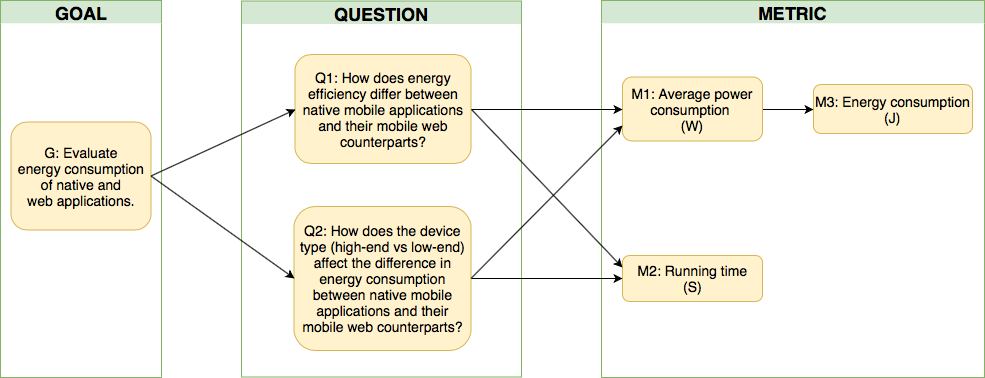
\includegraphics[width=\textwidth]{AppVSweb/figures/GQMtree.png}
\caption{\textcolor{blue}{GQM model hierarchical structure}}
\label{fig:GQMtree}

\end{figure*}
\\To present the experiment idea in a visual way, we picture a GQM tree (\autoref{fig:GQMtree}) based on the elements above.
%\afterpage{\clearpage}
